%%%%%%%%%%%%%%%%%%%%%%%%%%%%%%%%%%%%%%%%%
% Arsclassica Article
% LaTeX Template
% Version 1.1 (1/8/17)
%
% This template has been downloaded from:
% http://www.LaTeXTemplates.com
%
% Original author:
% Lorenzo Pantieri (http://www.lorenzopantieri.net) with extensive modifications by:
% Vel (vel@latextemplates.com)
%
% License:
% CC BY-NC-SA 3.0 (http://creativecommons.org/licenses/by-nc-sa/3.0/)
%
%%%%%%%%%%%%%%%%%%%%%%%%%%%%%%%%%%%%%%%%%

%----------------------------------------------------------------------------------------
%	PACKAGES AND OTHER DOCUMENT CONFIGURATIONS
%----------------------------------------------------------------------------------------

\documentclass[
12pt, % Main document font size
a4paper, % Paper type, use 'letterpaper' for US Letter paper
oneside, % One page layout (no page indentation)
%twoside, % Two page layout (page indentation for binding and different headers)
headinclude,footinclude, % Extra spacing for the header and footer
BCOR5mm, % Binding correction
]{scrartcl}
\usepackage{float}
%%%%%%%%%%%%%%%%%%%%%%%%%%%%%%%%%%%%%%%%%
% Arsclassica Article
% Structure Specification File
%
% This file has been downloaded from:
% http://www.LaTeXTemplates.com
%
% Original author:
% Lorenzo Pantieri (http://www.lorenzopantieri.net) with extensive modifications by:
% Vel (vel@latextemplates.com)
%
% License:
% CC BY-NC-SA 3.0 (http://creativecommons.org/licenses/by-nc-sa/3.0/)
%
%%%%%%%%%%%%%%%%%%%%%%%%%%%%%%%%%%%%%%%%%

%----------------------------------------------------------------------------------------
%	REQUIRED PACKAGES
%----------------------------------------------------------------------------------------

\usepackage[
nochapters, % Turn off chapters since this is an article        
beramono, % Use the Bera Mono font for monospaced text (\texttt)
eulermath,% Use the Euler font for mathematics
pdfspacing, % Makes use of pdftex’ letter spacing capabilities via the microtype package
dottedtoc % Dotted lines leading to the page numbers in the table of contents
]{classicthesis} % The layout is based on the Classic Thesis style

\usepackage{arsclassica} % Modifies the Classic Thesis package

\usepackage[T1]{fontenc} % Use 8-bit encoding that has 256 glyphs

\usepackage[utf8]{inputenc} % Required for including letters with accents

\usepackage{graphicx} % Required for including images
\graphicspath{{Figures/}} % Set the default folder for images

\usepackage{enumitem} % Required for manipulating the whitespace between and within lists

\usepackage{lipsum} % Used for inserting dummy 'Lorem ipsum' text into the template

\usepackage{subfig} % Required for creating figures with multiple parts (subfigures)

\usepackage{amsmath,amssymb,amsthm} % For including math equations, theorems, symbols, etc

\usepackage{varioref} % More descriptive referencing

%----------------------------------------------------------------------------------------
%	THEOREM STYLES
%---------------------------------------------------------------------------------------

\theoremstyle{definition} % Define theorem styles here based on the definition style (used for definitions and examples)
\newtheorem{definition}{Definition}

\theoremstyle{plain} % Define theorem styles here based on the plain style (used for theorems, lemmas, propositions)
\newtheorem{theorem}{Theorem}

\theoremstyle{remark} % Define theorem styles here based on the remark style (used for remarks and notes)

%----------------------------------------------------------------------------------------
%	HYPERLINKS
%---------------------------------------------------------------------------------------

\hypersetup{
%draft, % Uncomment to remove all links (useful for printing in black and white)
colorlinks=true, breaklinks=true, bookmarks=true,bookmarksnumbered,
urlcolor=webbrown, linkcolor=RoyalBlue, citecolor=webgreen, % Link colors
pdftitle={}, % PDF title
pdfauthor={\textcopyright}, % PDF Author
pdfsubject={}, % PDF Subject
pdfkeywords={}, % PDF Keywords
pdfcreator={pdfLaTeX}, % PDF Creator
pdfproducer={LaTeX with hyperref and ClassicThesis} % PDF producer
}

%----------------------------------------------------------------------------------------
%	BIBLIOGRAPHY
%----------------------------------------------------------------------------------------

\usepackage{biblatex} %Imports biblatex package
\addbibresource{sample.bib} %Import the bibliography file % Include the structure.tex file which specified the document structure and layout

\hyphenation{Fortran hy-phen-ation} % Specify custom hyphenation points in words with dashes where you would like hyphenation to occur, or alternatively, don't put any dashes in a word to stop hyphenation altogether

%----------------------------------------------------------------------------------------
%	TITLE AND AUTHOR(S)
%----------------------------------------------------------------------------------------

\title{\normalfont\spacedallcaps{Article Title}} % The article title

%\subtitle{Subtitle} % Uncomment to display a subtitle

\author{\spacedlowsmallcaps{Fabrizio Cominetti, Davide Abete, Ruben Agazzi}} % The article author(s) - author affiliations need to be specified in the AUTHOR AFFILIATIONS block

\date{} % An optional date to appear under the author(s)
\usepackage{hyperref}
%----------------------------------------------------------------------------------------

\begin{document}

%----------------------------------------------------------------------------------------
%	HEADERS
%----------------------------------------------------------------------------------------

\renewcommand{\sectionmark}[1]{\markright{\spacedlowsmallcaps{#1}}} % The header for all pages (oneside) or for even pages (twoside)
%\renewcommand{\subsectionmark}[1]{\markright{\thesubsection~#1}} % Uncomment when using the twoside option - this modifies the header on odd pages
\lehead{\mbox{\llap{\small\thepage\kern1em\color{halfgray} \vline}\color{halfgray}\hspace{0.5em}\rightmark\hfil}} % The header style

\pagestyle{scrheadings} % Enable the headers specified in this block

%----------------------------------------------------------------------------------------
%	TABLE OF CONTENTS & LISTS OF FIGURES AND TABLES
%----------------------------------------------------------------------------------------

\maketitle % Print the title/author/date block

\setcounter{tocdepth}{2} % Set the depth of the table of contents to show sections and subsections only

\tableofcontents % Print the table of contents


%----------------------------------------------------------------------------------------
%	ABSTRACT
%----------------------------------------------------------------------------------------

\section*{Abstract} % This section will not appear in the table of contents due to the star (\section*)

Il progetto realizzato consiste nella creazione di una base di dati a grafo contenente le relazioni fra i vari prodotti Marvel. All'interno del database sono presenti relazioni come ad esempio fra personaggi e fumetti, personaggi e personaggi, etc... 

%----------------------------------------------------------------------------------------
%	AUTHOR AFFILIATIONS
%----------------------------------------------------------------------------------------


%----------------------------------------------------------------------------------------

\newpage % Start the article content on the second page, remove this if you have a longer abstract that goes onto the second page

%----------------------------------------------------------------------------------------
%	INTRODUCTION
%----------------------------------------------------------------------------------------

\section{Introduzione}
Lo scopo del progetto consiste nella realizzazione di un database a grafo riguardante vari prodotti Marvel, fra cui personaggi, film, serie tv e fumetti.
L'obiettivo del progetto è di ottenere una sorta di "rete sociale" di super eroi o personaggi marvel, i quali sono collegati ai rispettivi fumetti, film , serie tv, o rispettivi collegamenti interpersonali fra personaggi e personaggi.
 
%----------------------------------------------------------------------------------------
%	METHODS
%----------------------------------------------------------------------------------------

\section{Fonti dati}
Per l'ottenimento dei dati sono stati utilizzati due metodi diversi: l'utilizzo di una Web API e Web Scraping.

\subsection{Web Scraping}
Per la parte riguardante il Web Scraping come sorgente dati è stata utilizata la Marvel Cinematic Universe Wiki.

Lo scraping è stato effettuato eseguendo un notebook python.
I passi eseguiti dal notebook per completare lo scraping sono:
\begin{enumerate}
\item Ottenimento dalla pagina relativa a tutti i personaggi della wiki i nomi dei personaggi con i relativi link alla pagina personale.
\item per ogni personaggio aprire la pagina personale e ottenere sempre tramite scraping le informazioni rilevanti, come ad esempio: biografia, lista di film in cui è presente il personaggio, lista di serie tv in cui è presente il personaggio e relazioni con altri personaggi.
\item Per ogni film trovato nelle pagine dei personaggi aprire la pagina relativa al film e ottenere tramite scraping le informazioni del film come ad esempio la trama, i registi, scrittori, compositori, incasso, data di uscita e durata del film.
\item Per ogni serie trovata nelle pagine dei personaggi aprire la pagina relativa alla serie e ottenere tramite scraping le informazioni della serie in questione, come ad esempio la trama, i registi, i produttori e i compositori
\item Salvataggio temporaneo all'interno di file csv di film, serie tv e personaggi per essere processati in seguito.
\end{enumerate}

\subsection{Web Api}
Per l'ottenimento dei dati tramite web API è stata utilizzato il servizio formito dalla Marvel che mette a disposizione una sua Web Api per ottenere i dati relativi a personaggi e fumetti.
L'ottenimento dei dati è avvenuto tramite esecuzione di un notebook python.
L'esecuzione consiste nei seguenti passi:
\begin{enumerate}
\item Ottenimento dei dati dei personaggi in formato JSON tramite chiamata al relativo endpoint della web api a gruppi di 100 personaggi, in quanto è il limite imposto dagli sviluppatori del servizio.
\item Salvataggio su file CSV dei dati relativi ai personaggi ottenuti, in modo da eseguire successive manipolazioni facilmente tramite la libreria \textit{pandas}, prima di inserire i dati nel database.
\item Ottenimento dei dati dei fumetti in formato JSON tramite chiamata al relativo endpoint della web api a gruppi di 100 fumetti, in quanto è il limite imposto dagli sviluppatori del servizio.
\item Salvataggio su file CSV dei dati relativi ai personaggi ottenuti , in modo da eseguire successive manipolazioni facilmente tramite la libreria \textit{pandas}, prima di inserire i dati nel database..
\end{enumerate}
\section{Data Exploration}
La fase di data exploration è stata realizzata sempre utilizzando python con alcune librerie grafiche per la creazione di visualizzazioni.

\subsection{Data Quality}
Le principali problematiche riscontrate nella qualità dei dati sono state riscontrate nelle biografie dei personaggi e nelle relazioni tra personaggi ottenute tramite web scraping;
\subsubsection{Data Quality e Cleaning Biografia}
Per quanto riguarda la qualità dei dati delle biografie le principali problematiche sono:
\begin{enumerate}
	\item Il notebook salva i vari paragrafi delle biografie come una lista di stringhe, quindi prima di tutto la biografia viene trasformata in una stringa, concatenando le varie stringhe presenti nella lista e inserendo un carattere newLine fra un elemento e l'altro.
	\item Il notebook inoltre salvava alcuni paragrafi della biografia più volte, per questo prima di concatenare la stringa viene effettuato un controllo per vedere se la porzione di stringa è già stata aggiunta alla stringa finale
	\item Infine viene fatto un escaping dei caratteri speciali, come ad esempio il carattere " o ', in modo da non avere problemi nell'inserimento nel database dei dati.
\end{enumerate}
\subsubsection{Data Quality e Cleaning Relazioni}
Per quanto riguarda la qualità dei dati delle relazioni interpersonali ottenute tramite web scraping la principale problematica consiste nell'assenza in alcune relazioni del nome del personaggio interessato, ad esempio ci sono relazioni che hanno come nome personaggio "Mother", "Father" e così via.
Per risolvere questa problematica il notebook esegue le seguenti operazioni:
\begin{enumerate}
	\item Per ogni personaggio vengono recuperate le relative relazioni.
	\item Per ogni relazione ottenuta viene effettuato un controllo sul nome del personaggio della relazione, se il nome non è presente all'interno della lista di personaggi la relazione viene scartata
\end{enumerate}
\begin{figure}[H]
  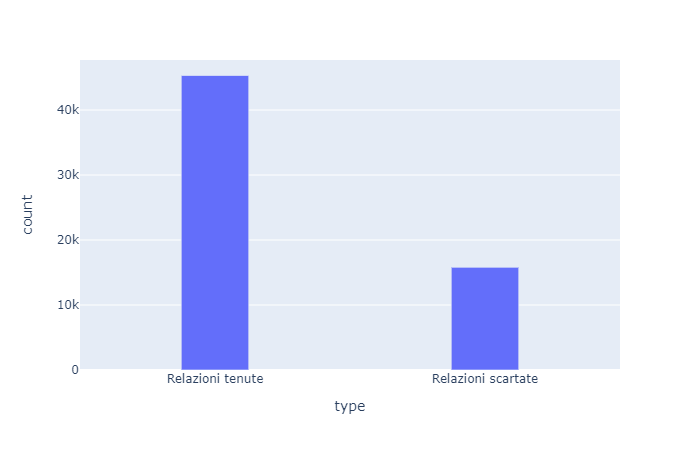
\includegraphics[scale=0.5]{plot_relazioni.png}
  \caption{Grafico relativo alle relazioni tenute rispetto a quelle scartate}
\end{figure}
\subsection{Completezza}
Sono state effettuate altre analisi riguardanti la completezza dei dati: in particolare al riguardo di attributi dei dati ottenuti.
\subsubsection{Dati personaggi}
Le analisi di completezza effettuate sui personaggi consistono nel confronto fra i dati ottenuti dalla web api e quelli ottenuti tramite web scraping. In particolare si può riscontrare una corrispondenza di 323 personaggi della web api con quelli ottenuti tramite web scraping, al netto dei 1559 personaggi della web api.
\begin{figure}[H]
  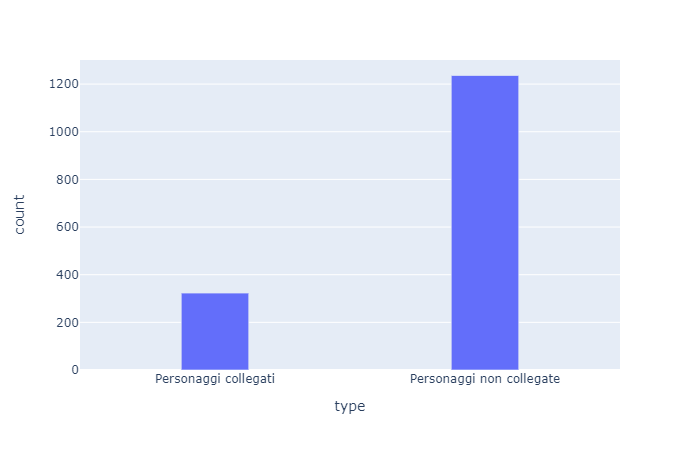
\includegraphics[scale=0.5]{plot_corrispondenza_personaggi.png}
  \caption{Grafico al numero di personaggi che sono collegabili con i dati ottenuti tramite web scraping.}
\end{figure}
\subsubsection{Descrizione fumetti}
Le analisi di completezza effettuate sulle descrizioni dei fumetti, ottenute tramite web api, consiste nel vedere quanti fumetti possiedono una descrizione. In particolare circa 19000 fumetti non hanno descrizione al netto dei circa 50000 fumetti.
\begin{figure}[H]
  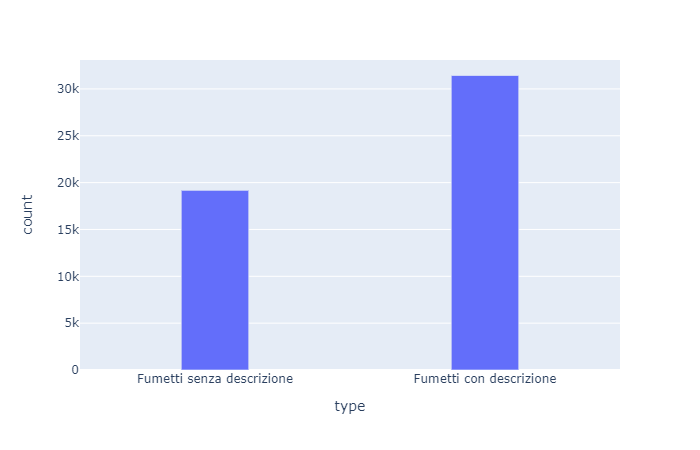
\includegraphics[scale=0.5]{plot_descrizione_fumetti.png}
  \caption{Grafico relativo al numero di fumetti con e senza descrizione}
\end{figure}
\section{Data Integration}
Per il processo di Data Integration sono state collegate dove possibile le due sorgeti dati tramite gli schemi dei personaggi, i quali fungono da punto di incontro fra le due sorgenti dati. è stata realizzata un operazione di record linkage fra i dati dei personaggi
\subsection{Data preparation}
Prima di tutto si aggiunge una nuova colonna al dataset del web scraping e della web api, contenente il nome del personaggio senza alcuni caratteri particolari come ad esempio " o ' e senza qualsiasi porzione di testo racchiusa fra delle parentesi. Queste operazioni sono state effettuate tramite l'utilizzo della libreria python "re" per pulire le stringhe. Le parentesi sono tolte per poter fare il confronto dei personaggi senza tenere conto in questo caso della singola variante del personaggio(ad esempio stesso personaggio di universi differenti). In output si avranno i due schemi relativi ai personaggi con un campo nome processato come detto precedentemente.
\subsection{Schema transformation}
Durante la fase di schema matching è stato effettuato un processo di reverse Engineering per capire cosa rappresentassero i dati della web api, non è stato fatto per lo scraping in quanto abbiamo scelto noi quali dati prendere e quindi lo schema era già chiaro a priori
L'analisi dello schema relativo ai personaggi è così composto:

\begin{enumerate}
	\item Id: identificativo univoco assegnato dall'api ad ogni personaggio
	\item description: Breve descrizione del personaggio
	\item modified: ultima modifica apportata al personaggio
	\item thumbnail: url che porta ad un immagine del personaggio
	\item comics: lista di fumetti in cui il personaggio è presente, con relativo id fumetto
	\item series: lista di serie di fumetti in cui il personaggio è presente
	\item stories: lista di storie in cui il personaggio è presente
	\item events: lista di eventi in cui ha partecipato il personaggio
	
\end{enumerate}

L'analisi dello schema relativo ai fumetti ottenuti tramite web api ha permesso di identificare i seguenti attributi:
\begin{enumerate}
	\item Id: identificativo univoco relativo al fumetto
	\item title: titolo del fumetto
	\item description: breve descrizione del fumetto
	\item modified: ultima modifica dei dati relativi al fumetto
	\item isbn, upc, diamondCode, ean, issn: identificativi editoriali relativi al fumetto
	\item forma: Formato di stampa del fumetto
	\item pageCount: numero di pagine del fumetto
	\item series: lista delle serie a cui appartiene il fumetto
	\item thumbnail: url relativa ad un immagine della copertina del fumetto
	\item images: url relativi a varie immagini del fumetto
	\item creators: lista dei creatori del fumetto
	\item characters: lista di personaggi appartenenti al fumetto
	\item stories: lista di storie appartenenti al fumetto
	\item events: lista di eventi significativi presenti nel fumetto
\end{enumerate}
%\begin{enumerate}
%\item Per ogni personaggio, sia proveniente da scraping che da web api, creo, se non esiste, un nodo <<character>> all'interno del database a grafo, utilizzando come discriminante sull'esistenza il nome processato generato nella fase di schema transformation. Se il nodo esiste già non faccio nulla.
%	\item Per ogni personaggio collego il nodo character corrispondente al nome processato ad un nodo <<character variant>>, che sara creato se non esiste, che è identificato tramite il nome vero e proprio non processato. Se il nodo esiste già procedo aggiungendo le informazioni aggiuntive relative al personaggio. 	
%\end{enumerate}
\subsection{Corrispondences Investigation}
Durante la fase di \textit{Corrispondences Investigation}, si è notato che si possono unire le due basi di dati sulla base dei personaggi, più specificatamente è possibile stabilire un collegamento fra i personaggi sulla base del loro nome. Dopo varie analisi si è notato che sia nel caso della base di dati ottenuta tramite consultazione della web api sia di quella ottenuta tramite web scraping, che un personaggio è identificato tramite un nome privo di parentesi e un'eventuale variante del personaggio è identificata da un nome all'interno della parentesi. Alla luce di queste considerazioni una regola di confronto fra i due schemi consiste nel vedere se due nomi di personaggi sono uguali dopo aver rimosso parentesi ed eventuali testi all'interno delle parentesi.
\subsection{Schemas Integration}
La fase di schemas integration avviene durante l'inserimento dei dati nel database: per ogni record presenti nei due schemi relativi ai personaggi vengono rimosse le porzioni di stringa contenute all'interno di parentesi tramite l'utilizzo della libreria \textit{re}; in seguito viene creato all'interno del database un nodo di tipo \textit{character} se non è già presente un nodo dello stesso tipo con lo stesso nome. Al nodo character, sia che è stato creato oppure no, viene collegato un nodo \textit{Character Variant} identificato tramite nome completo, ovvero il nome prima della rimozione delle parentesi, contenente tutte le informazioni presenti nel record personaggio in esame. Ovviamente anche il nodo \textit{Character Variant} viene creato solo se non esiste già, mentre se esiste vengono solo aggiunte informazioni mancanti presenti nella base di dati da cui proviene il personaggio in esame.
\section{Database}
Il database scelto per lo starage dei dati è un database a grafo. i motivi che hanno portato a questa scelta sono:
\begin{enumerate}
	\item Dati non in real time: la mole di dati riguardante l'universo marvel non è enorme e non necessita di un inserimento di dati real time, quindi le operazioni di scrittura sono relativamente poche e le operazioni in lettura sono molte di più; proprio per questo un database a grafo può essere utilizzato in quanto lento in scrittura ma veloce in lettura.
	\item Lo scopo del dataset è mostrare le varie relazioni fra i prodotti marvel e quindi un database a grafo è l'ideale, in quanto è basato sul concetto di relazioni e collegamenti
\end{enumerate}
\subsection{Struttura Database}
La struttura del database è la seguente:
\subsubsection{Nodi}
I nodi presenti all'interno del database sono:
\begin{enumerate}
	\item Comic: nodo rappresentante un fumetto Marvel, con al suo interno il suo id fumetto ottenuto dall'api, i vari codici di identificazione,come ad esempio ISBN, la descrizione del fumetto se è presente, il formato del fumetto e il numero di pagine.
	\item Movie: nodo rappresentante un film Marvel, con al suo interno i vari dati relativi al film come ad esempio la trama del film, i registi, scrittori, produttori, compositori, incassi, durata del film, e data di rilascio del film
	\item Tv Show: nodo rappresentante una serie tv Marvel, con al suo interno i vari dati relativi al film come ad esempio la trama della prima stagione, i registi, gli showrunner, produttori, compositori.
	\item Character: nodo rappresentante la versione generica di un personaggio, contiene al suo interno il nome del personaggio
	\item Character Variant: Nodo che rappresenta una variante precisa di un personaggio, contenente informazioni come ad esempio il nome, una descrizione del personaggio e una biografia del personaggio.
\end{enumerate}
\subsubsection{Relazioni}
Le relazioni presenti fra i nodi all'interno del database sono:
\begin{enumerate}
	\item In Film: relazione che collega un nodo <<Character Variant>> ad un nodo film, rappresenta appunto la partecipazione del personaggio all'interno del film
	\item In Serie: relazione che collega un nodo <<Character Variant>> ad un nodo ts show, rappresenta la partecipazione del personaggio all'interno di una serie tv.
	\item In fumetto: relazione che collega un nodo <<Character Variant>> ad un nodo <<Comic>>, rappresenta la partecipazione del personaggio all'interno di un fumetto.
	\item Conosce: relazione che collega un nodo <<Character Variant>> ad un nodo <<Character Variant>>, rappresenta una relazione inter-personale fra due personaggi.
	\item <<Variante di>>: relazione che rappresenta una variante di un personaggio base, collega un nodo di tipo <<character>> ad un nodo di tipo <<character variant>>.
\end{enumerate}

\subsection{Statistiche database}
All'interno del database sono stati creati in totale $60411$ nodi distribuiti nel seguente modo: 

\begin{center}
\begin{tabular}{||c c||} 
 \hline
 Etichetta Nodo  & Numero Di Nodi \\ [0.5ex] 
 \hline\hline
	
	Character & 4609 \\ \hline 
	Character Variant & 5113 \\ \hline
	Comic & 50607 \\ \hline
	Movie & 43 \\ \hline
	Tv Show & 19 \\ [0.5ex] \hline 
\end{tabular}
\end{center}
Fra i nodi del database sono state create $117763$ relazioni distribuite nel modo seguente
\begin{center}
\begin{tabular}{||c c||} 
 \hline
 Etichetta Relazione  & Numero Di Relazioni \\ [0.5ex] 
 \hline\hline
	Conosce & 19040 \\ \hline 
	In Film & 531 \\ \hline
	In Serie & 2405 \\ \hline
	In Fumetto & 90503 \\ \hline
	Variante di & 5284 \\ [0.5ex] \hline 
\end{tabular}
\end{center}
\begin{figure}[H]
  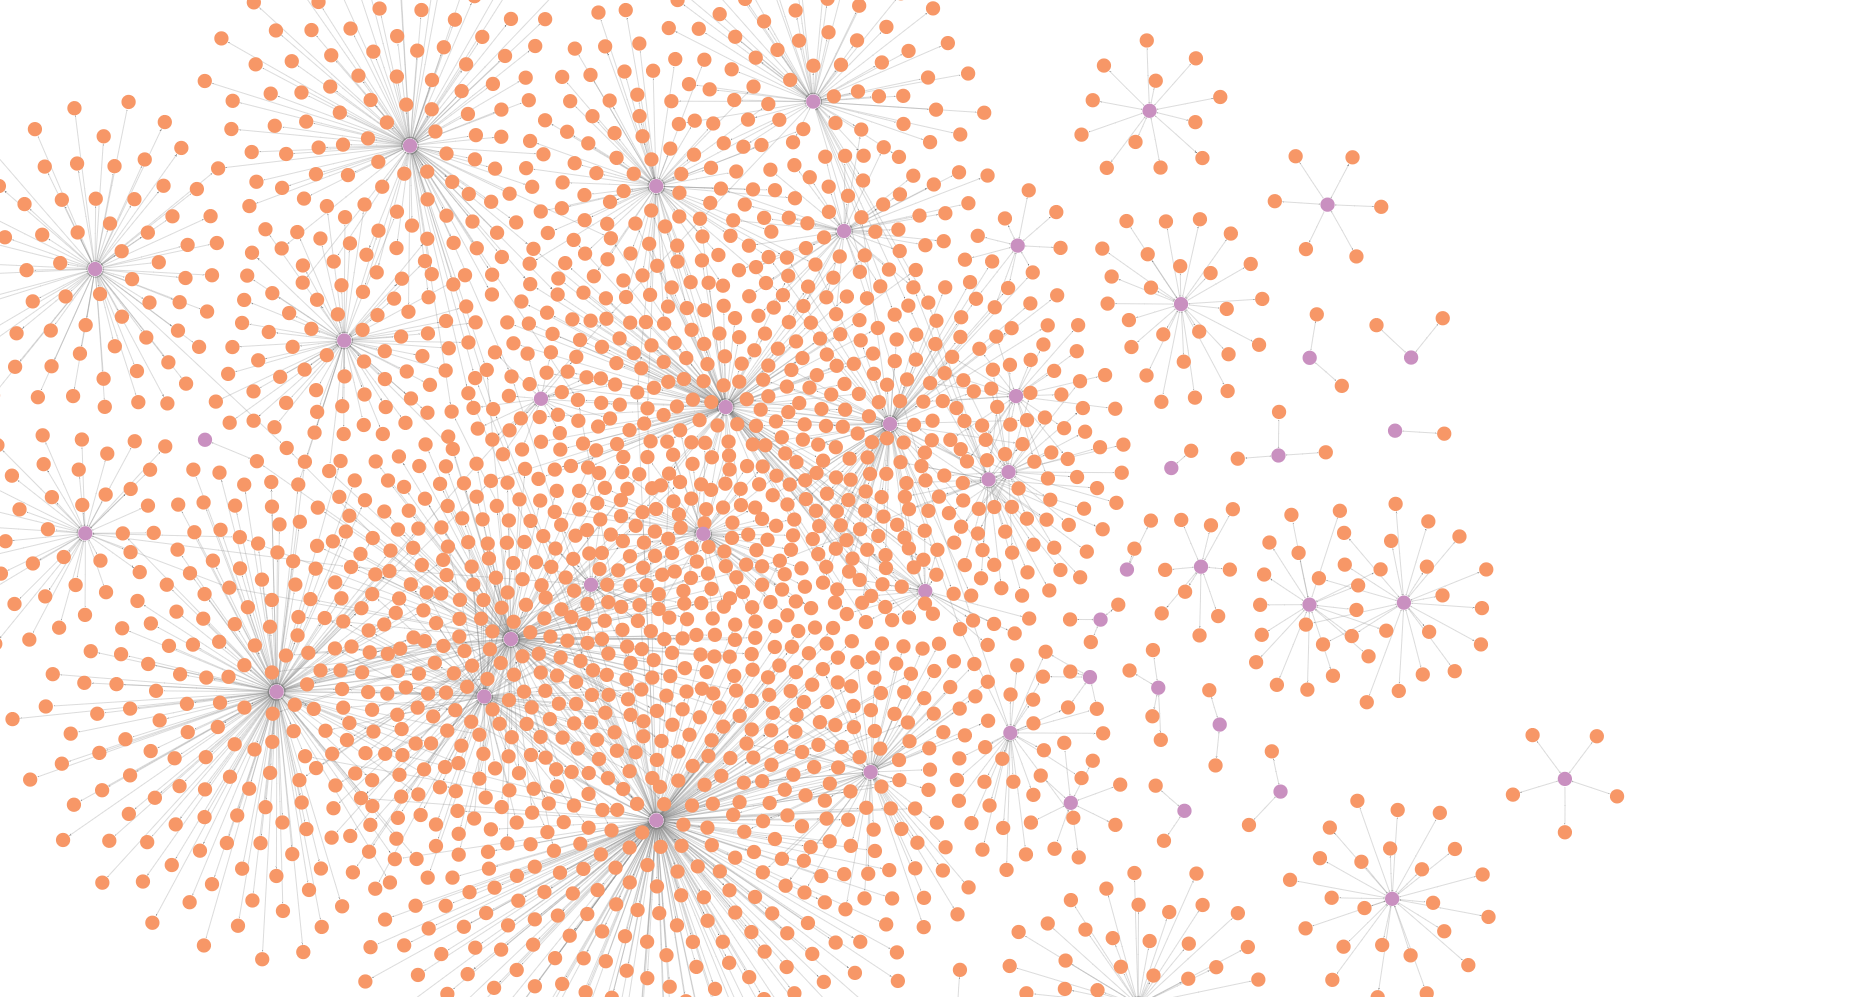
\includegraphics[scale=0.27]{./Figures/comic-variant.png}
  \caption{Visualizzazione di alcuni nodi Character variant(Viola) in relazione a dei nodi Comic(Arancione)}
\end{figure}
\subsection{Alcune Query}
 Grazie alla struttura a grafo del database è possibile ottenere 
 facilmente tramite query relazioni fra i nodi. Ad esempio potremmo 
 trovare i personaggi conosciuti dal personaggio "Iron Man",
  che sono presenti nel film \textit{Avengers}. 
	Per ottenere questo risultato si può utilizzare la seguente query 
	CYPHER: \\\newline \textit{MATCH (i:character\_variant)-[r:conosce]->(c:character\_variant)-[p:in\_film]\\->(m:movie) WHERE i.name = "Iron Man"  AND m.title = "The Avengers" RETURN i,r,c,p,m} 

%----------------------------------------------------------------------------------------
%	RESULTS AND DISCUSSION
%----------------------------------------------------------------------------------------


%----------------------------------------------------------------------------------------
%	BIBLIOGRAPHY
%----------------------------------------------------------------------------------------

\renewcommand{\refname}{\spacedlowsmallcaps{References}} % For modifying the bibliography heading

\bibliographystyle{unsrt}

\bibliography{sample.bib} % The file containing the bibliography

%----------------------------------------------------------------------------------------

\end{document}